\chapter{Внешний вид}

\section{Что внешний вид способен рассказать о вас?}

\textit{Источник: \url{https://thewallmagazine.ru/what-does-the-look-tell-adout-you/}}

\textit{Автор: Анна Радионова}

\begin{flushright}
    \it Как-то во время индивидуальной беседы она втолковывала одной ученице, что внешность не имеет значение — куда важнее твоя личность. «Какую только чушь не приходится вдалбливать в детские головы», — думала Тесса, листая журнал.

    Джоан Роулинг. Случайная вакансия
\end{flushright}

Тема внешности во все времена являлась довольно деликатной и вызывающей жаркие споры среди представителей обоих полов. Кто-то делал выводы о человеке за первые 30 секунд знакомства и  придерживался мнения о том, что его визуальный образ способен как позитивно, так и негативно влиять на его жизнь. Иные, напротив, считали, что внутренний мир непременно важнее внешней оболочки, и глупо осуждать человека за независящие от него вещи. Каждый и по сей день придерживается той или иной точки зрения в большей степени, и что интересно, сторонники обеих правы.

Для того чтобы продолжать разговор о внешнем виде, стоит прояснить получившуюся путаницу, из-за которой происходит столкновение двух позиций, которые по своей сути не являются противоречащими. Следует понимать, что понятия внешности и внешнего вида в корне различны. Внешность – это то, что дано природой, тогда как внешний вид – то, что формирует сам человек и то, за что ответственен только он. А значит встречать и «судить» человека по его внешнему виду не только непредосудительный, но и весьма полезный навык, особенно, если в сферу профессиональных обязанностей входит подбор персонала, или просто есть желание чуть лучше разбираться в людях и  производить на окружающих приятное впечатление.

\begin{fancyquotes}
    Внешность – это то, что дано природой, тогда как внешний вид – то, что формирует сам человек и то, за что ответственен только он
\end{fancyquotes}

Существует ряд особенностей в манере одеваться, заметив которые, можно делать выводы о некоторых чертах характера человека, которого решили «встретить по одёжке».

Во-первых, необходимо смотреть на общую ухоженность человека: в каком состоянии ногти и волосы, аккуратно ли он одет, выглажена ли одежда, нет ли на ней пятен. Немаловажно и то, как он пахнет.[1] Конечно, по какому-либо одному пункту, вроде мятой рубашки, не стоит вешать на человека ярлык неряхи, однако, если есть два и более, то это может свидетельствовать о низкой самооценке и серьёзной внутренней дисгармонии. (Важно не приравнивать аккуратность и ухоженность к наличию у человека дорогих вещей известных брендов и возможности каждую неделю посещать салон красоты, так как это больше имеет отношение к материальному состоянию, нежели личным качествам человека.)

Что же касается следования модным тенденциям, безропотное их соблюдение говорит о том, что человек зависим от мнения окружающих и одежда помогает ему чувствовать себя частью сообщества.

Манера одеваться слишком сексуально и вызывающе может свидетельствовать о том, что у человека, предпочитающего такой стиль, как минимум, острый недостаток внимания, и подобные проявления – не что иное, как попытка выделиться из толпы и заявить о себе. Однако также это может быть свидетельством эмоционального и сексуального неблагополучия.

Люди, предпочитающие, кричаще яркие цвета и броские аксессуары, как правило, страдают от неуверенности в себе. Они остро нуждаются во внимании окружающих, что нередко может быть объяснено их низкой самооценкой.

Другая крайность – слишком унылые расцветки и чересчур консервативный покрой вещей говорят о застенчивости их обладателя. Такие люди предпочитают оставаться в тени, в стороне от внимания, стремясь таким образом защититься от проблем.

Идеально сидящая одежда и аккуратно причёсанные волосы (у женщин, как правило, собранные) говорят о том, что перед нами человек высокоорганизованный и дисциплинированный. Аккуратность может свидетельствовать и о ряде негативных черт характера, таких как излишняя жёсткость, суровость, неумение уступать и идти на компромисс.

Одежда, несоответствующая случаю, может свидетельствовать о том, что это, вероятнее всего, неуверенный в себе человек, стремящийся к вниманию и создающий себе бунтарский образ. Такие люди стремятся к тотальному контролю над ситуацией и роли лидера в коллективе.

Также многое может сказать о человеке его причёска:

Мужчины, пытающиеся скрыть лысину, зачёсывая волосы набок, или тонирующие седину, как правило, являются неуверенными и скрытными натурами, не готовыми откровенничать и выдавать всю правду о себе.

Женщины же, часто меняющие причёску и цвет волос, постоянно находятся в поиске индивидуальности и наиболее комфортного образа, что также может свидетельствовать о неуверенности в себе и низкой самооценке.

Необычные прически говорят о том, что их обладатель буквально кричит о своем желании быть замеченным. Тогда как чересчур консервативные прически «волосок к волоску» говорят о негибкости и неумении уступать.

Согласно последним исследованиям учёных, внешние данные, заложенные природой, тоже могут служить источником информации о человеке. Например, исследователи из Чехии утверждают, что нашли зависимость между чертами лица и уровнем интеллекта. [2]

По их мнению, для людей с более высоким уровнем интеллекта характерны далеко посаженные глаза, крупный нос, приподнятые уголки губ и заострённый подбородок.  Что интересно, по утверждению самих учёных, полученные данные применимы только к мужской аудитории, и уровень интеллекта женщины таким образом определить нельзя.

Учёные из Университета Эдинбурга пошли дальше и определили зависимость между симметричностью лица и прошлым человека. В ходе продолжительного исследования было выявлено, что люди, в чьём детстве не было серьёзных испытаний и потрясений, обладают значительно более симметричными чертами лица, чем люди, столкнувшиеся в раннем возрасте с трудностями. [3]

\begin{fancyquotes}
    В ходе продолжительного исследования было выявлено, что люди, в чьём детстве не было серьёзных испытаний и потрясений, обладают значительно более симметричными чертами лица, чем люди, столкнувшиеся в раннем возрасте с трудностями
\end{fancyquotes}

А в Университете Глазго попробовали пересмотреть традиционные методы оценивания физической формы человека. По мнению шотландских учёных, гораздо большее значение для здоровья имеет не количество жировой ткани в организме человека, а то, в каких местах она откладывается. Так, например, пухлые щёчки могут свидетельствовать о большей подверженности человека стрессам и инфекционным заболеваниям. [4]

Таким образом, не остается сомнений, что внешний вид – это не просто картинка, на которую не стоит обращать внимание. Напротив, стоит, но главное, не забывать, что внешность – это оружие, и оно выстрелит, только если внутри есть патроны.

[1-4]  \url{https://thewallmagazine.ru/what-does-the-look-tell-adout-you/}


\newpage
\section{Можно ли определить характер человека по внешности?}

\textit{... и как это сделать}

\textit{Источник: \url{https://dzen.ru/a/YIl6ixA3r08hfeqe}}

Мы нередко льстим себе, считая, что с одного взгляда способны понять человека. На поверку оказывается, внешность обманчива, а первое впечатление ничего общего не имеет с действительностью. И все-таки наука физиогномика утверждает, что можно определить характер человека по внешности. Для этого нужно обратить внимание на отдельные черты лица, понять, о чем свидетельствует их формы и размеры. Объединив полученные сведения, можно создать целостный образ. Разберемся в азах этой науки.

\textbf{Физиогномика — китайское учение о «чтении» внешности}

Учение об определении характера человека по внешним признакам возникло в Китае. Оно существует столетия, и за это время официальная наука не смогла ни подтвердить, ни опровергнуть его постулаты. Главный принцип физиогномики: в человеке все взаимосвязано — и внешнее, и внутреннее, поэтому особенности характера буквально «написаны на лице». Если научиться читать эти признаки, можно легко разобраться, с кем вы имеете дело.

Физиогномисты считают, что мышцы лица постоянно отвечают на сигналы нервной системы человека и сокращаются под их воздействием. На протяжении многих лет такой работы мышцы привыкают к определенному положению, и это формирует пропорции. Все мы считываем информацию с внешности, но делаем это неосознанно, потому часто заблуждаемся относительно внутренних качеств людей.

\begin{fancyquotes}
    Физиогномика --- метод определения типа личности человека, его душевных качеств и состояния здоровья, исходя из анализа внешних черт лица и его выражения.\\

    Виды физиогномики: 1. изучение невербального поведения (мимики, телесной моторики); 2. изучение особенностей лица — физиогномики, строения тела.\\

    \begin{flushright}
        \texttt{https://ru.wikipedia.org/wiki/Физиогномика}
    \end{flushright}
\end{fancyquotes}

Чтобы определять характер человека по внешности, нужно научиться мгновенно считывать особенности лица, обращать внимание на глаза, уши, нос. Это поможет больше узнать о темпераменте, типе мышления, понять мотивы поступков других людей. Есть нюанс: женские лица трудно читать из-за косметики. Впрочем, основные пропорции определить можно, а это уже немало.

\textbf{На что обратить внимание, чтобы определить характер человека по внешности}

По мнению физиогномистов, важнейших черт лица всего три: глаза, брови, нос. Именно они передают наибольшее количество информации о человеке. Также много говорят форма рта, губы и уши. Давайте научимся читать самые выразительные черты.

\textbf{Старая истина: глаза — зеркало души}

Есть много данных о том, как цвет глаз отображает характер человека, но это противоречивая и спорная информация, а в эпоху моды на цветные контактные линзы еще и бесполезная. Лучше остановимся на форме и размере глаз:

\begin{enumerate}
    \item Большие глаза указывают на чувствительность и мужественность. А обладатели маленьких глаз нередко упрямы, ревнивы, самодовольны.
    \item Опущенные уголки глаз свидетельствуют об оптимизме, добродушии. Приподнятые — о чувствительности, смелости, решительности.
    \item Если верхнее веко наползает на середину глаза, человек ловок и проницателен. А если веко провисает целиком, это свидетельствует о сексуальной привлекательности, но холодности.
    \item Провисающее нижнее веко говорит о душевной теплоте, а разбухшее посередине — об эгоцентричности.
\end{enumerate}

\begin{figure}
    \centering
    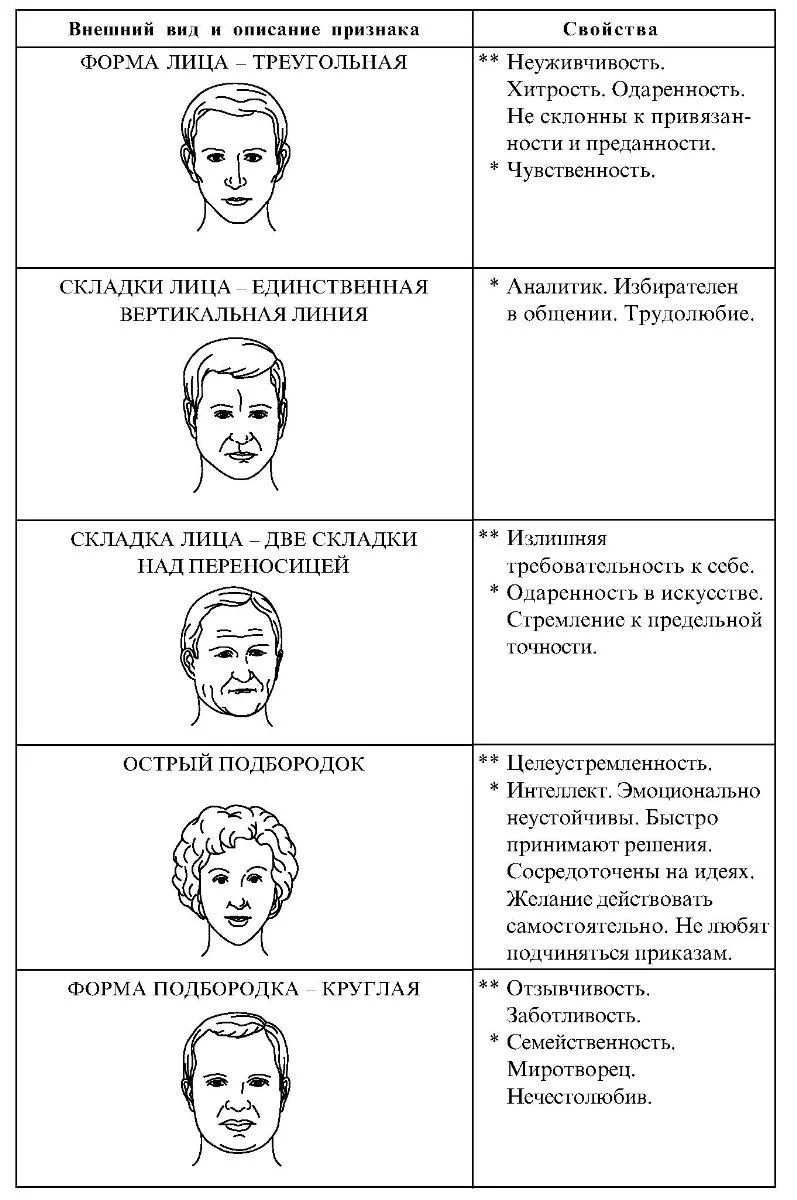
\includegraphics[width=0.6\textwidth]{img/faces.png}
    \caption{Обратите внимание, если оба века выглядят отечными, это тревожный признак: человек устал от жизни или нездоров.}
\end{figure}

\textbf{Читаем особенности характера мужчины по бровям}

Женские брови часто подвергаются косметической коррекции, поэтому по ним трудно судить о чертах характера. А вот мужские могут многое рассказать об обладателе. В первую очередь следует обратить внимание на толщину бровей. Чем она больше, тем упрямее человек. Важен конец брови: тонкий свидетельствует о благородстве, широкий может говорить мужественности и даже жесткости, отличных предпринимательских качествах.

Если бровь заметно длиннее глаза, перед вами человек с гибким умом, а в целом длинные брови говорят о спокойном и несколько консервативном характере. Грубые и короткие брови часто свидетельствуют о влюбчивости и непостоянстве натуры. Также короткие и густые брови бывают о вспыльчивых, агрессивных и самодостаточных людей. Форма бумеранга указывает на изобретательность.

\begin{figure}[h]
    \centering
    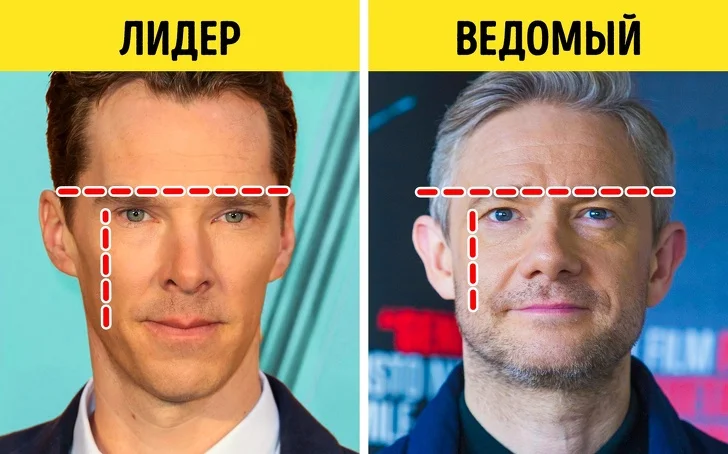
\includegraphics[width=0.5\textwidth]{img/brows.png}
    \caption{Люди, у которых почти отсутствуют брови, закрыты и хитры. Крупные сросшиеся «моноброви» — у решительных, прямолинейных и смекалистых натур. Если внутри брови видна родинка, человек легко добивается целей.}
\end{figure}

\textbf{Правда ли, что длинный нос характерен для лгунов?}

Нет, это сказка. Очень большая длина носа указывает на ум, капризность, а умеренно длинные носы у консервативных людей. Если нос еще широкий, то человек спокоен и устойчив. А короткие носы у дружелюбных открытых оптимистов.

Костлявый нос говорит о плохой концентрации внимания, но если он с горбинкой, то это может указывать на гордый, решительный, упрямый характер, иногда даже агрессивность. Такой нос у женщины свидетельствует, что она конкурентоспособна в мужском коллективе, амбициозна. А маленький нос нередко бывает у ревнивых натур.


\begin{figure}
    \centering
    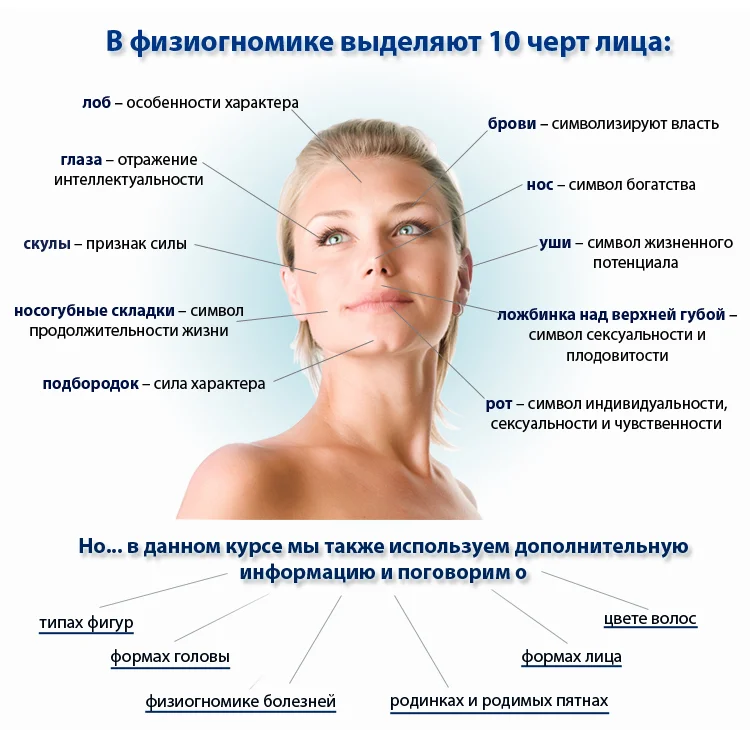
\includegraphics[width=0.65\textwidth]{img/face2.png}
    \caption{В физиогномике выделяют 10 черт лица.}
\end{figure}


Обратите внимание на форму кончика носа:
\begin{enumerate}
    \item Круглая — благополучная натура, умеющая быть счастливой в любых обстоятельствах.
    \item Отвисшая — признак сексуальности.
    \item Заостренная — склонность к непостоянству, предательству.
    \item Выпуклая — свидетельство душевной теплоты.
    \item Похожая на орлиный клюв — мстительность.
    \item Вздернутый нос говорит о сексуальной раскрепощенности, неумении хранить тайны.
\end{enumerate}

Понимание, что означают те или иные особенности носа, дает возможность мгновенно оценить многие свойства характера.

\textbf{Главное о чтении характера человека по внешности}

Помните, что:
\begin{enumerate}
    \item Физиогномика не точная наука, а только учение китайских мудрецов. Не стоит придавать ей излишнего значения.
    \item Современные косметические процедуры творят чудеса. Читая по лицу человека, особенно женщины, легко ошибиться.
    \item Нередки пластические операции. О том, что они вообще были, вы можете узнать только от самого человека.
    \item Черты лица меняются. В зависимости от того, какие мышцы чаще всего задействуются, зависит выражение лица, его особенности. Некоторые черты становятся более выраженными, а какие-то — менее.
\end{enumerate}

Лицо, руки и пальцы многое могут рассказать о человеке, но не следует делать скоропалительных выводов, не пообщавшись с ним.

